\documentclass[a4paper,12pt]{article}
%For links
%\usepackage{url}
%For images
\usepackage{graphicx}
\begin{document}
\begin{enumerate}
   \item 

   \item Följande bild och beskrivning finns i en Volvo V70 instruktionsbok:
   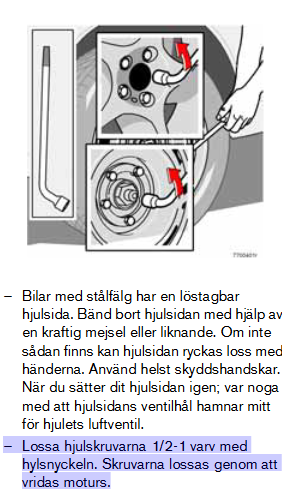
\includegraphics{Figur.png}

    Denna instruktion handlar om hur man lossar på ett hjul, men samma principer
    kan gå åt motsatt håll när man försöker dra åt 
    Hylsnyckelns längd kan uppskattas till några decimeter, vi säger 2. Då gäller det att vrida
    bulten 1 varv, vilket krävs för att dra åt den helt. 

    Newtons/grad * 360 grader 


    \item Vid kastbanans högsta punkt så är hastigheten för y axeln 0. Detta är för att
    kulan är precis vid sin maxpunkt och är påväg att börja åka neråt på grund utav
    graviationskraften.

    Istället kan endast hastigheten på x-axeln räknas ut enkelt så här:
    $22*cos(27^\circ)=20 m/s$ vilket då också är den totala hastigheten vid den punkten.

    \item För att simplifiera problemet kan man vinkla flaggstången så den liknar
    en gungbräda. Då får vi följande diagram:
    
    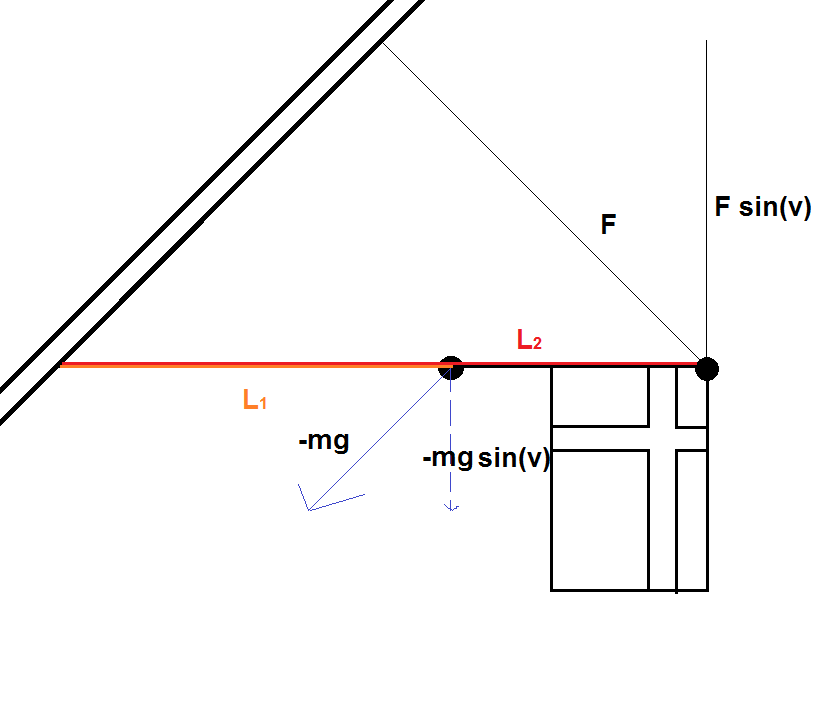
\includegraphics[scale=0.55]{Figur2.png}
    
    Flaggstången är i jämnvikt, så genom momentlagen får vi att summan av vridmomenten
    blir noll.

    $$FL_2sin(v)-mgL_1sin(v)=0$$
    $$FL_2=mgL_1$$
    $$F==\frac{mgL_1}{L_2}$$

    I uppgiften får vi reda på att massan på flaggstången är 53kg, Längden till 
    tyngpunkten är 5 meter från punkten och att hela flaggstångens längd
    är 8.4 meter. Då får vi att F = 310 N.

\end{enumerate}
\end{document}